\documentclass{beamer}
\usepackage[T1]{fontenc}
\usepackage[ansinew]{inputenc}
\usepackage{%
  booktabs,
  ngerman,
  amsmath,
  nicefrac,
  bbm,
  graphicx
}

\newcommand{\abs}[1]{\ensuremath{\lvert#1\rvert}}
\usetheme{TUDO}
\let\epsilon=\varepsilon

\title[useR 2008 / \texttt{desiRe}]{Desirabilitiy functions in \\
  multicriteria optimization \\[1em]
  \large Observations made while implementing \texttt{desiRe}}
%% Andere Autoren einf�gen
\author[O.~Mersmann]{%
  Olaf~Mersmann
  \and Heike~Trautmann
  \and Detlef~Steuer
  \and Claus~Weihs
  \and Uwe~Ligges}
\institute[TU Dortmund]{Fakult�t f�r Statistik / TU Dortmund}
\logo{\includegraphics[width=3cm]{tud_logo_rgb}}

\begin{document}
%% ============================================================
\begin{frame}
  \titlepage
\end{frame}

\begin{frame}
  \frametitle{Multicriteria Optimization Problem}
  \begin{block}{Given:}
    \def\arraystretch{1.5}
    \begin{tabular}{ll}
      Influence factors & $X=(X_1,\dotsc, X_n)'$ \\
      Objectives        & $Y_1,\dotsc, Y_k$  with $Y_i = f_i(X_1,\dotsc, X_n, \epsilon_i)$ \\
    \end{tabular}
  \end{block}
  \begin{block}{Goal:}
    \[
    \min_{X_1,\dotsc,X_n} (Y_1,\dotsc,Y_k)
    \]
    possibly given some restriction functions
  \end{block}
\end{frame}

\begin{frame}
  \frametitle{Desirabilities}
  \begin{block}{Idea}
    Map objective values to $[0, 1]$. Interpret 1 as \emph{desirable} and 0 as
    \emph{undesirable}
  \end{block}
  \vskip1em
  \begin{block}{Types}
    \begin{description}
      \item[One-sided] Objective value should be as above or below a threshold
      \item[Two-sided] Objective value should stay in between two thresholds
    \end{description}
  \end{block}
  \vskip1em
  \begin{block}{Applications}
    \begin{itemize}
    \item Mostly in chemistry, chemical and mechanical engineering
    \item Optimization of production- or chemical processes
    \item Quality Control 
    \end{itemize}
  \end{block}
\end{frame}

\begin{frame}
  \frametitle{Harrington Desirabilities}
  \begin{columns}[c]
    \column[T]{.5\textwidth}
    \begin{block}{One-Sided}
      \centerline{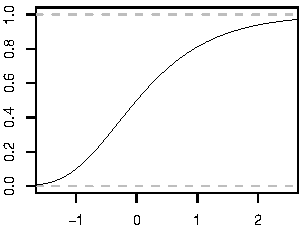
\includegraphics{h1.pdf}}
      \vskip-2em
      \begin{align*}
        d(Y_i') &= \exp(-\exp(-\abs{Y_i'}^{n_i})) \\
        Y_i'      &= b_0 + b_1Y_i
      \end{align*}
      Parameters: $b_0$, $b_1$
    \end{block}
    \column[T]{.5\textwidth}
    \begin{block}{Two-Sided}
      \centerline{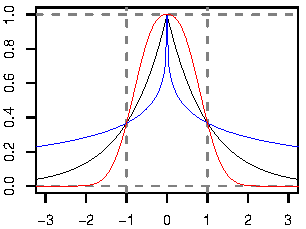
\includegraphics{h2.pdf}}
      \vskip-2em
      \begin{align*}
        d(Y_i') &= \exp(-\abs{Y_i'}^{n}) \\
        Y_i'      &= \frac{2Y_i - (USL + LSL)}{USL - LSL}
      \end{align*}
      Parameters: $LSL$, $USL$, $n$
    \end{block}
  \end{columns}
\end{frame}

\begin{frame}
  \frametitle{Derringer-Suich Desirabilities}
  \begin{columns}[c]
    \column[T]{.5\textwidth}
    \begin{block}{One-Sided}
      \centerline{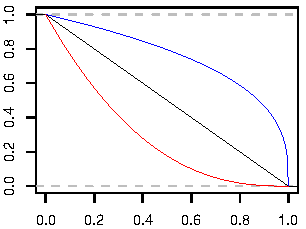
\includegraphics{d1.pdf}}
    \end{block}
    \column[T]{.5\textwidth}
    \begin{block}{Two-Sided}
      \centerline{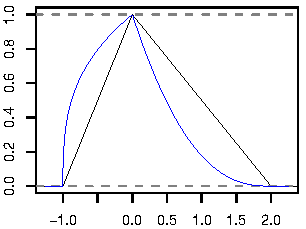
\includegraphics{d2.pdf}}
    \end{block}
  \end{columns}
\end{frame}

\begin{frame}
  \frametitle{Desirability Index (DI)}
  \begin{block}{Geometric DI}
    \[ D_g := (\prod_{i=1}^k d_i^{w_i})^{1/\sum w_i} \]
  \end{block}
  \begin{block}{Minimum DI}
    \[ D_{\min} := \min_{1\le i \le k} d_i \]
  \end{block}
  \begin{block}{Mean DI}
    \[ D_{m} := \frac1k \sum_{i=1}^k d_i \]
  \end{block}

  Solve MCO by maximizing appropriate DI
\end{frame}

\begin{frame}
  \centerline{\bfseries\Large Demonstration}
\end{frame}

\begin{frame}
  \frametitle{Things not shown:}
  \begin{itemize}
    \item Explicit \texttt{d/p/q/r} functions for Harrington and Derringer-Suich desirabilities
    \item Control Chart functions (\emph{in progress})
    \item Plot functions
    \item Generalized Derringer-Suich desirabilities
    \item Linearization of Derringer-Suich desirabilities
  \end{itemize}
\end{frame}

%\begin{frame}
%  \frametitle{Things planned:}
%\end{frame}

\begin{frame}
  \frametitle{Where to get it}
  \begin{center}
  \texttt{\large http://r-forge.r-project.org/projects/desire/}
  \vskip2em
  or
  \vskip2em
  {\large CRAN (\emph{coming soon})}
  \end{center}
\end{frame}
\end{document}

%%% Local Variables:
%%% mode: latex
%%% TeX-master: t
%%% fill-column:90
%%% End:
